\documentclass[a4paper,10pt]{article}
\usepackage[utf8]{inputenc}
\usepackage[brazilian]{babel}
\usepackage{cite}
\bibliographystyle{plain}
\usepackage{hyperref}
\usepackage{indentfirst}
\usepackage{url}
\usepackage{graphicx}
\usepackage{wrapfig}
\usepackage{caption}
\usepackage{amsmath}
\usepackage{enumerate}
\usepackage{placeins}

%opening
\title{RELATÓRIO 1 - VARIÁVEIS ESPAÇOS-TEMPORAIS DA MARCHA}
\author{Camila Takano, Damiana A. Santos, João Oda}

\begin{document}

\maketitle

\begin{abstract}
Este relatório descreve o procedimento experimental e os resultados obtidos na primeira experiencia da disciplina Princípios e Aplicações de Biomecânica, Turma: EN2308
\end{abstract}

\section{Introdução}
As medidas espaço temporais da marcha podem ser adquiridas de forma simples possibilitando uma primeira analise do movimento e constituindo uma fonte importante de informação.

\section{Método}

\subsection{Participantes}
Neste experimentos foram obtidos dados de três indivíduos na faixa etária 20 a 30 anos, denominados doravante \textbf{C}, \textbf{D} e \textbf{J}. Sendo \textbf{C} e \textbf{D} do sexo feminino e \textbf{J} do sexo masculino. 

\subsection{Procedimento Experimental}
O comprimento do membro inferior dos participantes foi medido, sendo a distância do 
Maléolo Medial até Espinha Ilíaca Ântero-Superior.

Uma região de 15m de comprimento foi delimitada, por onde os participantes andam em trajetória aproximadamente retilínea a uma velocidade hipoteticamente constante, para atingir a velocidade constante um trecho de 5m é previamente percorrido. Ao tocar com o pé na região delimitada, inicia-se a cronometragem de tempo e a contagem de passos(a partir do $1^o$) ao pisar fora da região para-se se o cronômetro e a contagem de passos é encarrada. Cada um dos participantes é submetido a este procedimento três vezes, cada vez com uma ritmo/velocidade(Lento, Confortável e Rápido)

\section{Resultados}

Os dados medidos são apresentados na tabela \ref{tab_medidas}, exceto o comprimento $L$ do membro inferior que se encontra na tabela \ref{tab_calculados}. Calculou-se então a cadência de passos($CD$), o comprimento do passo($CP$) e a velocidade do andar($Va$ e $Vb$), estes dados se apresentam na tabela \ref{tab_calculados}. Os cálculos foram realizados segundo as formulas:

\begin{equation}
\label{eq_CD}
 CD = \frac{N_p}{t}
\end{equation}

\begin{equation}
\label{eq_CP}
CP = \frac{d}{N_p}
\end{equation}

\begin{equation}
 \label{eq_Va}
 Va = \frac{d}{t}
\end{equation}

\begin{equation}
\label{eq_Vb}
Vb = CP \times CD 
\end{equation}

Sendo $d$ a distância percorrida, $N_p$ o número de passos e $t$ tempo gasto. Desta forma ressaltamos que os valores calculados são valores médios para o percurso.

A variação de $CD$ e $CP$ em função de $Va$ são apresentados respectivamente nos gráficos \ref{plotCDxVa} e \ref{plotCPxVa}.

Os dados foram normalizados com relação ao comprimento do membro inferior($L$) e tornados adimensionais seguindo:
\begin{equation}
CP_{norm} = \frac{CP}{L}
\end{equation}
\begin{equation}
CD_{norm} = CD \sqrt{\frac{L}{g}}
\end{equation}
\begin{equation}
Va_{norm} = \frac{Va}{\sqrt{gL}}
\end{equation}


Os valores normalizados são apresentados na tabela \ref{tab_norm} e podem ser visualizados na
figura \ref{plotNorm}

\begin{table}
\begin{center}
\begin{tabular}{l|ccc|ccc}
 & \multicolumn{3}{|c|}{N$^o$ de Passos} & \multicolumn{3}{|c}{Tempo(s)}\\
 velocidade & \textbf{C} & \textbf{D} & \textbf{J} & \textbf{C} & \textbf{D} & \textbf{J}\\
 \hline
Lenta & 26 & 26 & 24 & 14.06 & 13.66 & 17.37\\
Confortável & 24 & 24 & 18 & 10.94 & 12.44 & 12.66\\
Rápida & 18 & 20 & 14 & 7.91 & 8.97 & 6.82
\end{tabular}
\end{center}
\caption{Dados Medidos}
\label{tab_medidas}
\end{table}

\begin{table}
\begin{center}
\begin{tabular}{ll|lcccc}
&L(m)&velocidade & CD(passos/s) & CP(m) & Va(m/s) & Vb(m/s)\\
\hline
 & &Lenta & 1.85 & 0.58 & 1.07 & 1.07\\
\textbf{C}& 0,8&Confortável & 2.19 & 0.62 & 1.37 & 1.37\\
 & &Rápida & 2.28 & 0.83 & 1.90 & 1.90 \\
\hline
 & &Lenta & 1.90 & 0.58 & 1.10 & 1.10\\
\textbf{D}& 0,82&Confortável & 1.93 & 0.62 & 1.21 & 1.21\\
 & &Rápida & 2.23 & 0.75 & 1.67 & 1.67\\
\hline
 & &Lenta & 1.38 & 0.62 & 0.86 & 0.86\\
\textbf{J}& 1,0&Confortável & 1.42 & 0.83 & 1.18 & 1.18\\
 & &Rápida & 2.05 & 1.07 & 2.20 & 2.20\\
\end{tabular}
\end{center}
\caption{Variáveis Calculadas}
\label{tab_calculados}
\end{table}

%e & $CD_{norm}$ & $CP_{norm$) & $Va_norm$ \\


\begin{table}
\begin{center}
\begin{tabular}{l|ccc|ccc|ccc}
& \multicolumn{3}{|c|}{$CD$} & \multicolumn{3}{|c}{$CP$} & \multicolumn{3}{|c}{$Va$}\\
velocidade & \textbf{C} & \textbf{D} & \textbf{J} & \textbf{C} & \textbf{D} & \textbf{J} & \textbf{C} & \textbf{D} & \textbf{J} \\ \hline
Lenta & 0.53 & 0.55 & 0.44 & 0.72 & 0.70 & 0.62 & 0.38 & 0.39 & 0.28\\
Confortável & 0.63 & 0.56 & 0.45 & 0.78 & 0.76 & 0.83 & 0.49 & 0.43 & 0.38\\
Rápida & 0.65 & 0.64 & 0.66 & 1.04 & 0.91 & 1.07 & 0.68 & 0.59 & 0.70
\end{tabular}
\end{center}

\caption{Variáveis Normalizadas}
\label{tab_norm}
\end{table}




\begin{figure}[h]
 \centering
 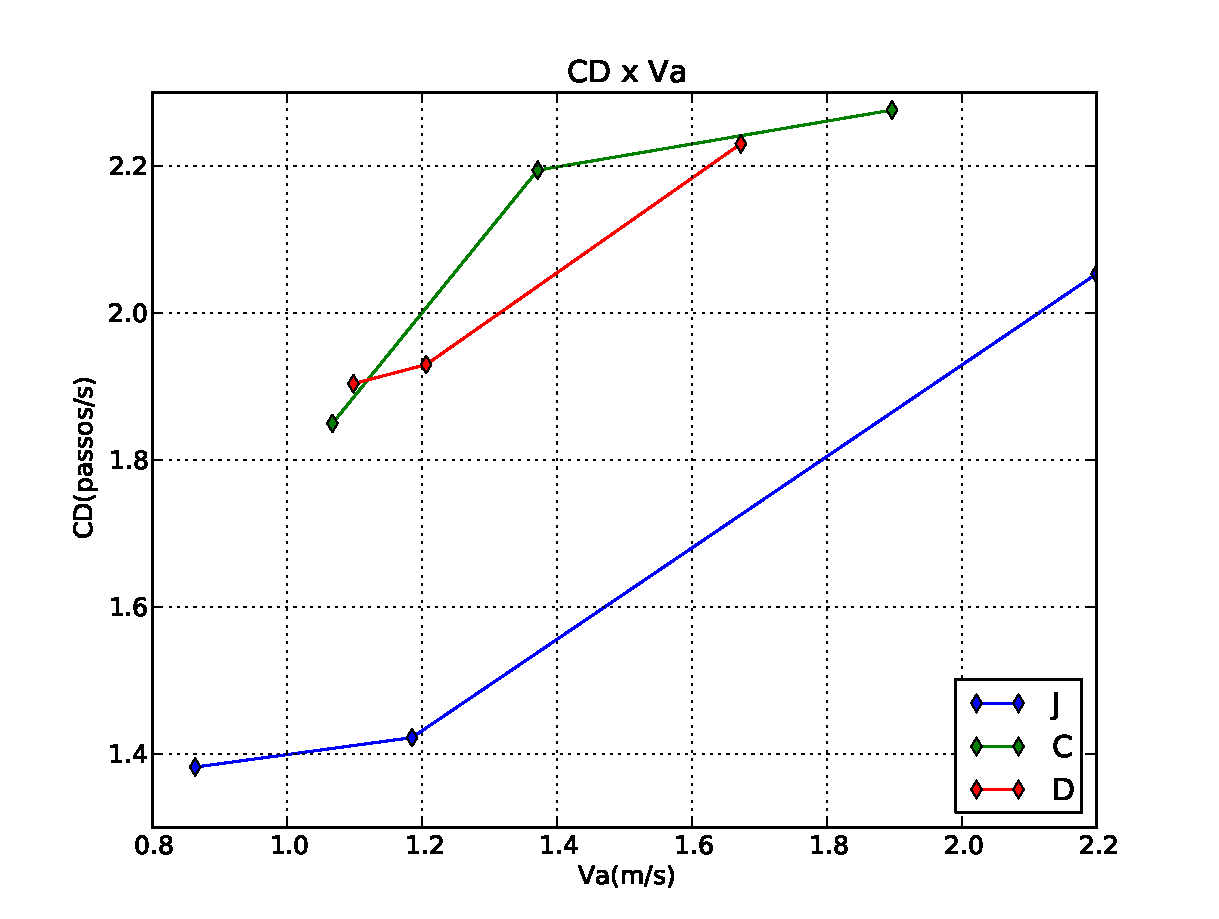
\includegraphics[scale=0.5,keepaspectratio=true]{./plot_CDxVa.pdf}
 % plot_CDxVa.pdf: 585x441 pixel, 72dpi, 20.64x15.56 cm, bb=0 0 585 441
 \caption{Gráfico Cadência de passos(CD) pela Velocidade do Andar(Va)}
 \label{plotCDxVa}
\end{figure}

\begin{figure}[h]

 \centering
 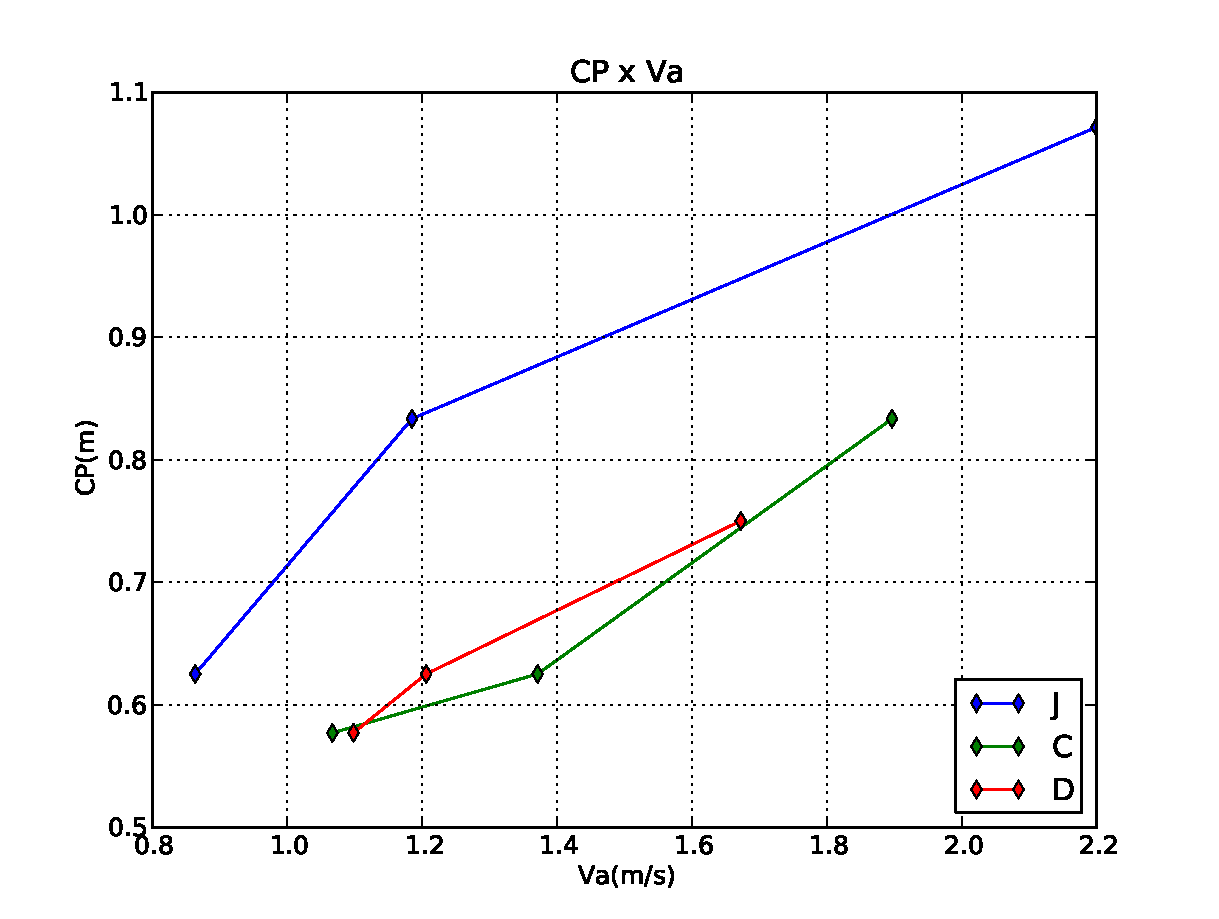
\includegraphics[scale=0.5,keepaspectratio=true]{./plot_CPxVa.pdf}
 % plot_CDxVa.pdf: 585x441 pixel, 72dpi, 20.64x15.56 cm, bb=0 0 585 441
 \caption{Gráfico Comprimento do passos(CP) pela Velocidade do Andar(Va)}
 \label{plotCPxVa}
\end{figure}

\begin{figure}[h]
 \centering
 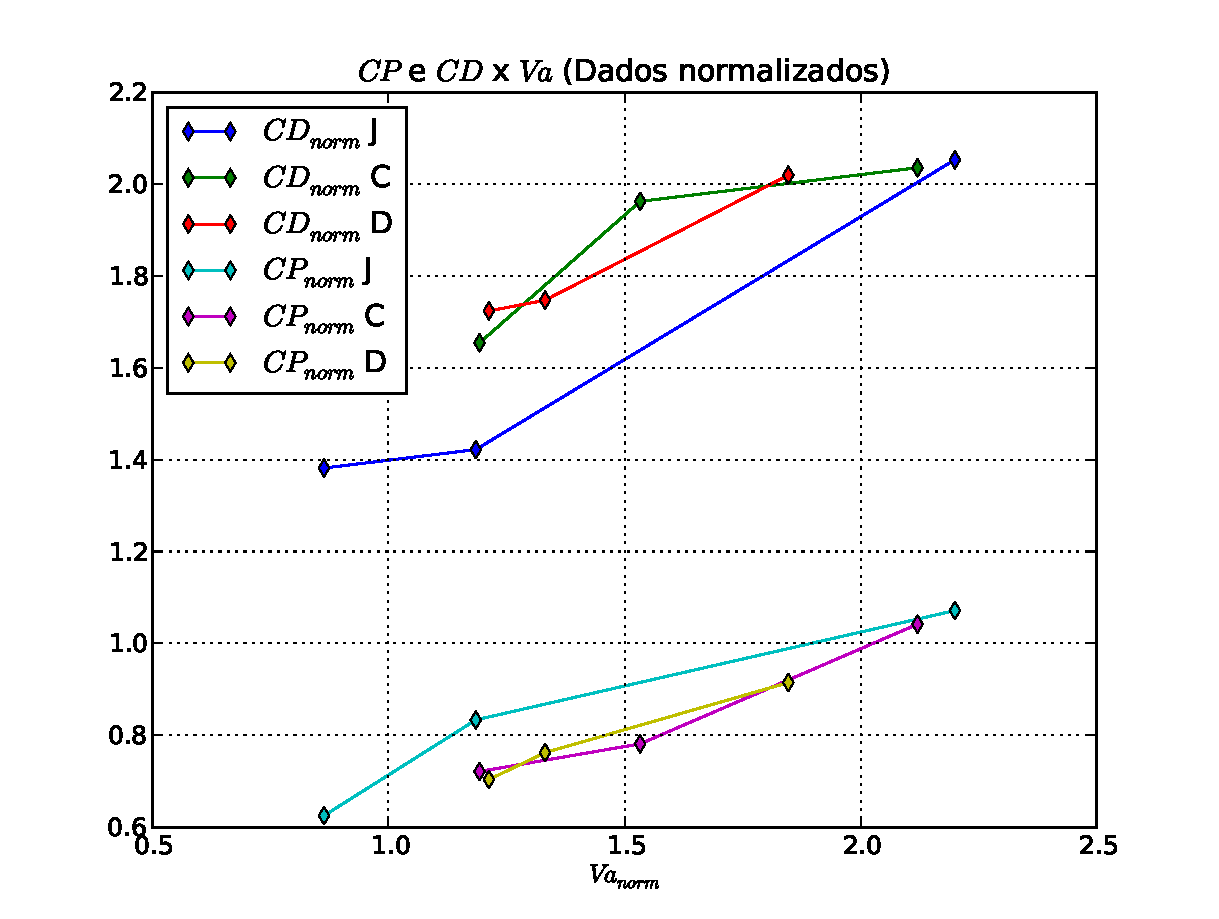
\includegraphics[scale=0.6,keepaspectratio=true]{./plot_Norm.pdf}
 % plot_Norm.pdf: 585x441 pixel, 72dpi, 20.64x15.56 cm, bb=0 0 585 441
 \caption{Gráfico da cadência de passos e comprimento do passo em função da velocidade do andar, todos os dados estão normalizados e são adimensionais}
 \label{plotNorm}
\end{figure}


\FloatBarrier
\section{Discussão}

\subsection{Dados Brutos e Normalizados}
Observando os dados brutos podemos perceber que em geral as sequências de pontos dos indivíduo \textbf{C} e \textbf{D} estão mais próximas entre si do que quando comparadas com a do indivíduo \textbf{J}


\subsection{Questões Propostas}
\subsubsection{Existe alguma relação entre CP e CD com o aumento de velocidade?}
As variáveis $CP$ e $CD$ estão relacionadas com a velocidade, a medida que a velocidade aumenta as variáveis também aumentam. Isto é um fato para todas as observações intra-indivíduos.

\subsubsection{Compare os resultados encontrados para Va e Vb, existiu diferença? Comente.}
Não houve diferença para $Va$ e $Vb$. pelas próprias formulas(\ref{eq_CD} \ref{eq_CP} \ref{eq_Va} \ref{eq_Vb}) utilizadas observamos:

\begin{equation}
   Vb = CP \times CD = \frac{d}{N_p} \frac{N_p}{t} = \frac{d}{t} = Va
\end{equation}

\subsubsection{Comente a respeito dos erros de medida e dê sugestões de como diminuí-los (pense em soluções simples e também na utilização de instrumentos para, por exemplo, uma melhor quantificação do tempo decorrido).}

Houve um pequeno erro de medição para a distância total de percurso (15m), pois a ferramenta utilizada(trena) para medir essa distância não atingiu o comprimento desejado(um valor maior que o percurso). Sendo assim, faz-se importante verificar antes da realização do experimento se há equipamentos adequados para a realização dos mesmos.

A demora, mesmo que mínima(pelo menos o tempo de reação do ser humano), em iniciar e/ou parar o cronômetro podem ter ocasionado erros de cronometragem. Assim, seria interessante a utilização de equipamentos como sensores que iniciam e/ou param o cronômetro logo que um dos lados dos pés se posiciona no local desejado.

O conhecimento dos os métodos de análise do experimento pode influenciar os voluntários no desempenho da tarefa. 

O principal erro é de natureza sistemática, proveniente do procedimento adotado para medir a distância percorrida, esta foi considerada constante(15m), porem a distância percorrida é em geral maior, porem não mais do que o comprimento de dois passos.

A dificuldade do indivíduo em manter uma velocidade constante e sem mudança de direção nos três ritmos de velocidade (lento, confortável e rápido) pode ocasionar erros de medição. A utilização de câmeras de vídeo ou fotográficas de uma forma sistemática podem proporcionar maior clareza e detalhes durante a observação da marcha, minimizando os erros de medição do experimento.

Uma solução simples que poderiam contornar algum destes erros seria andar sobre um papel, proveniente por exemplo de um rolo de de papel pardo, com a sola dos pés/calçados recoberta com tinta fresca ou alguma outra alguma outra forma de rastrear as pegadas dos indivíduo.

\end{document}
